\chapter{Introduction}
\label{cha:Introduction}

\section{What is Spatial Audio?}

Spatial audio refers to a variety of technologies and techniques that aim to mimic the spatial characteristics of sound in the real space and apply those in the virtual space. These characteristics include the distance, direction and movement of a sound source, as well as the acoustics of the environment in which the sound is originating from. Compared to the usual stereo audio, spatial audio is far more effective in communicating where a sound is coming from and how far away it is. 

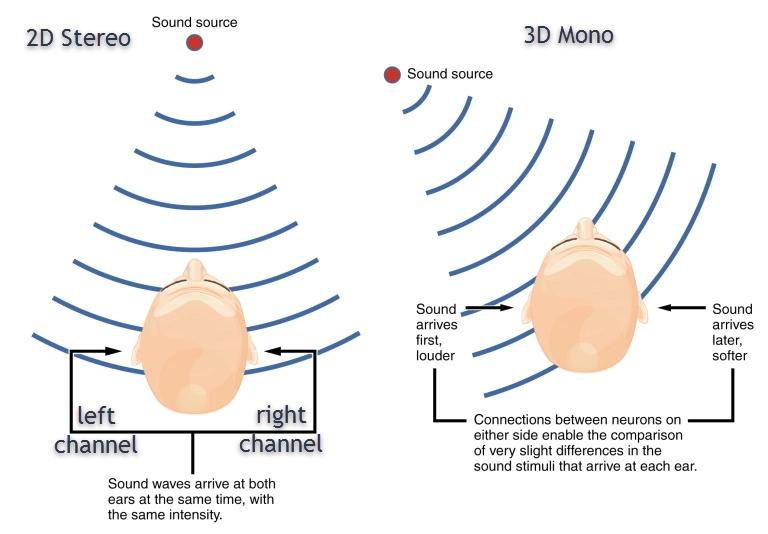
\includegraphics[width=.85\textwidth]{2DSoundVs3DSound}

In everyday life, humans are able to identify the location of a sound, even without seeing where exactly it came from. For example, a person can hear footsteps approaching from behind or recognize a dog barking in a nearby room. The human auditory cues, which help with the sound localization, are based on monaural and binaural cues. Monaural cues are processed individually in one ear, while binaural cues result from the comparison of sounds reaching the two ears. These mechanisms can help the brain estimate where the sound is coming from and to some extend figure out the elevation and distance of the sound source. More on this can be found in \cite[Chapter 3]{Carlini1}

In video games, spatial audio can greatly help with the perception of the virtual environment. Sounds can communicate the position of the object that is emitting the sound to the player, which in turn helps the player understand their surroundings without being able to see them. For example, the sound of walking and weapons clanking from a nearby room can suggest that an armed enemy is close. Spatial properties such as distance, direction, reverberation and sound obstruction can greatly support both environmental awareness and immersion for the player.